\section{La simulazione computerizzata}
Per riuscire ad orientarsi nel vasto panorama dei modelli esistenti inerenti il problema dell'evacuazione di folle, è necessario innanzitutto capire quali sono i principali criteri secondo cui ognuno di essi può essere classificato. \newline
La prima grande separazione può essere effettuata definendo le categorie \textit{macroscopico} e \textit{microscopico}, infatti, mentre un modello macroscopico non è costruito a partire dal pedone ma simula il comportamento dell'intera folla come un'unica entità, un modello microscopico analizza le azioni delle singole persone a livello locale e, dai loro apporti individuali, determina il movimento globale della folla. \newline
Un'altra differenziazione riguarda le modalità con cui vengono gestiti spazio e tempo all'interno dell'ambiente di simulazione. Specificatamente, la scelta verte tra l'opzione computazionalmente più vantaggiosa del \textit{discreto} e quella del \textit{continuo}, sovente più fedele alla realtà da simulare. \newline
Mentre i modelli macroscopici considerano i pedoni come tutti uguali tra loro, vista l'impossibilità di analizzare il singolo individuo, i modelli di tipo microscopico possono differenziarsi in \textit{eterogenei} ed \textit{omogenei}, per enfatizzare la possibilità o meno di rappresentare all'interno della folla persone che presentano caratteristiche distinte.

\subsection{Approcci esistenti}
Analizzando i principali modelli di simulazione delle folle presenti allo stato dell'arte \cite{Duives2013} \cite{Zheng2009}, è possibile individuare delle analogie nelle metodologie con cui questi sono stati formulati. In particolare, è possibile identificare quattro distinte tipologie di approccio, le cui principali caratteristiche sono riassunte nella tabella \ref{table:models-comparison}. 

\begin{table}
\centering
\renewcommand{\arraystretch}{1.5}
\begin{tabular}{|c|c|c|c|}
\hline
\textbf{Modello}            & \textbf{Tipologia} & \textbf{Spazio e Tempo} & \textbf{Pedone} \\ \hline
\textbf{Automi cellulari}   & Microscopico       & Discreto                & Omogeneo        \\ \hline
\textbf{Forze sociali}      & Microscopico       & Continuo                & Eterogeneo      \\ \hline
\textbf{Basati sull'agente} & Microscopico       & Discreto/Continuo       & Eterogeneo      \\ \hline
\textbf{Fluidodinamici}     & Macroscopico       & Continuo                & Omogeneo        \\ \hline
\end{tabular}
\caption{Tabella comparativa delle tipologie di modello di evacuazione di folle.}
\label{table:models-comparison}
\end{table}

\subsubsection{Automi cellulari}
Un automa cellulare è un sistema dinamico discreto, in cui lo spazio è rappresentato mediante una griglia di celle mentre il tempo da intervalli temporali prestabiliti. \newline
A partire da una configurazione in cui il sistema si trova ad una determinata iterazione, è possibile ottenere la successiva applicando l'insieme di regole costitutive del modello. Una regola ha lo scopo di modificare lo stato di ogni cella della griglia in relazione allo stato di quelle ad essa adiacenti. \newline
Nel caso dell'evacuazione di una folla, ad esempio, è possibile rappresentare i pedoni come celle oscurate e definirne il movimento tramite lo spostamento in una delle otto posizioni ad essa adiacenti, considerando l'eventuale presenza di altri pedoni e la vicinanza all'uscita. \newline
La semplicità concettuale che caratterizza questo tipo di modelli li rende sia computazionalmente molto efficienti sia adatti ad analizzare l'evoluzione di varie categorie di sistemi, da quelli biologici a quelli fisici. \newline
L'approssimazione di una qualsiasi entità con una cella però, in molte situazioni può risultare troppo riduttiva e poco descrittiva del problema in esame.

\subsubsection{Forze sociali}
Proposto per la prima volta da D. Helbing e P. Molnar \cite{Helbing1995}, il modello forze sociali si basa sull'assunzione che il movimento dei pedoni, apparentemente visto come un processo caotico, è il risultato dell'apporto di diversi fattori quali: la volontà di raggiungere una destinazione, mantenere una distanza da eventuali ostacoli o essere attratti dagli altri individui presenti. \newline 
Ognuno di questi stimoli, chiamati appunto \i{forze sociali}, susciterebbe nel pedone delle diverse reazioni, dipendenti dalle intenzioni di ognuno a compiere una piuttosto che l'altra azione e la cui combinazione determina la velocità e la direzione del movimento in ogni istante.

\subsubsection{Ad agenti}
I modelli basati sugli agenti approssimano il sistema con un insieme di entità capaci di interagire con i propri simili e di prendere delle decisioni autonome sulla base di un insieme di regole. \newline
Ogni agente ha il proprio stato interno, che può variare nel corso della simulazione in risposta a determinati eventi e lo rende riconoscibile rispetto a tutti gli altri. Le sue capacità relazionali, inoltre, permettono l'emergere di fenomeni che non si riscontrerebbero valutando separatamente il comportamento dei singoli. \newline 
Per queste loro caratteristiche, i modelli ad agenti si rivelano particolarmente flessibili ad essere arricchiti con nuovi livelli di dettaglio, grazie ai quali è possibile avvicinarsi sempre più ad una simulazione fedele alla realtà. \newline
Spesso, il loro principale limite, risiede nella difficoltà a scalare verso l'alto il numero di agenti presenti nella simulazione.

\subsubsection{Fluidodinamici}
A differenza dei precedenti, i modelli fluidodinamici sono di tipo macroscopico e si basano sull'assunzione che il movimento della folla è molto simile allo scorrimento di un fluido. \newline
Come sottolineato da Hughes \cite{Hughes2002}, questa formulazione, per essere considerata attendibile, richiede una densità di pedoni molto alta, altrimenti non si potrebbe giustificare l'uso delle equazioni di Navier-Stokes\n{\url{http://web.archive.org/web/20190522071242/https://www.comsol.it/multiphysics/navier-stokes-equations}}, le cui ipotesi sono quelle di modellare un continuo deformabile. \newline
L'utilizzo di questo tipo di approccio si rileva molto utile in casi analoghi al sopracitato pellegrinaggio alla Mecca, dove l'elevatissimo numero di presenti rende proibitivo l'impiego degli altri modelli. \newline
L'aspetto limitante risiede nel fatto che la precisione dei modelli fluidodinamici è vincolata alla quantità di pedoni presenti nella folla, che, se non sufficientemente alto, comporta una approssimazione troppo grossolana.

\subsection{Il modello IMPACT}
Il problema della maggior parte dei modelli esistenti è che essi rivolgono la loro attenzione principalmente sulle leggi fisiche e le forze in gioco nella simulazione, considerando i pedoni come particelle invece che come entità con caratteristiche socio-culturali peculiari ed una componente emotiva facilmente influenzabile da quella dei propri vicini \cite{Zheng2009}. \newline
Il modello ad agenti IMPACT \cite{vanderWal2017Model} nasce con l’obiettivo di analizzare l'importanza di questi aspetti, che vengono valutati all'interno di simulazioni inerenti l'evacuazione a causa di un incendio da un hub di trasporto.

\subsubsection{Network Oriented Modeling}
Per definire l'evoluzione dei processi emotivi dei pedoni viene usato l'approccio del Network Oriented Modeling \cite{Treur2018}. Questa scelta permette di descrivere attraverso un grafo orientato processi interconnessi tra loro e viene utilizzata nei più svariati ambiti, dalla biologia alla sociologia. \newline 
Ogni caratteristica che si desidera rappresentare costituisce un nodo del grafo, il cui stato $y(t)$ varia nel tempo secondo la seguente equazione differenziale:

\begin{equation*}
    \frac{dy(t)}{dt} = \eta_{y}[c_{y}(w_{x_1,y} \cdot x_1(t),...,w_{x_k,y} \cdot x_k(t)) - y(t)]
\end{equation*}

che in versione discreta può essere riscritta come

\begin{equation*}
    y(t + \Delta t) = y(t) + \eta_{y}[c_{y}(w_{x_1,y} \cdot x_1(t),...,w_{x_k,y} \cdot x_k(t)) - y(t)]\Delta t
\end{equation*}

dove $\eta_{y}$ è un fattore moltiplicativo utile a regolare la velocità dell'evoluzione, le $x_i(t)$ sono gli stati dei processi che influenzano l'aggiornamento di $y(t)$ e $c_{y}$ é la funzione che decide come devono essere combinati i vari $x_i(t)$ moltiplicati per i rispettivi pesi $w_{i,y}$.

\begin{figure}[ht]
  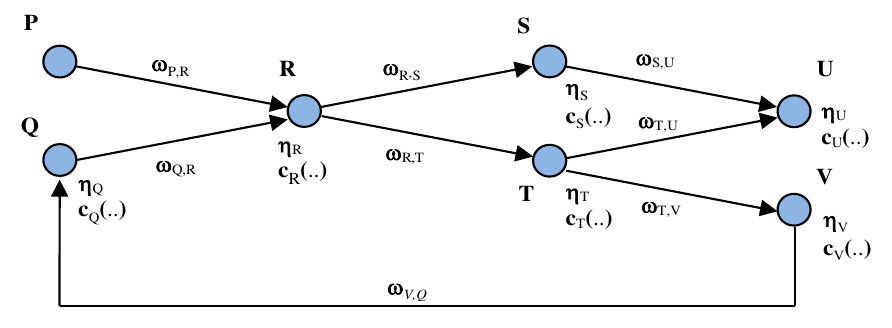
\includegraphics[width=\linewidth]{immagini/network-oriented-modeling.png}
  \caption{Esempio di Network Oriented Modeling rappresentato mediante grafo: i nodi contrassegnati con le lettere da P a V sono gli stati dei processi presi in considerazione, che vengono aggiornati valutando la provenienza e i pesi $w_{P..V,P..V}$ degli archi entranti utilizzando la rispettiva funzione di combinazione $c_{P..V}$.}

  \label{fig:net-model}
\end{figure}

\subsubsection{Risultati delle simulazioni}
Per determinare il reale impatto dei vari fattori presi in considerazione è stato utilizzato, come ambiente rappresentante un hub di trasporto, uno spazio quadrato di lato $20m$ con un'uscita in corrispondenza ad ognuno dei quattro muri ed un incendio nelle vicinanze del centro. Tale scelta, piuttosto semplice, ha l'obiettivo di ridurre al minimo il rischio che eventuali motivi strutturali, possano compromettere l'analisi della rilevanza delle caratteristiche descritte nel modello, che invece, in questo modo, rappresentano la principale fonte di variabilità all'interno della simulazione. \newline
Tra i vari aspetti presi in considerazione, il contagio sociale, fenomeno psicologico che porta al diffondersi di comportamenti, atteggiamenti o convinzioni comuni tra persone a contatto tra loro, si è dimostrato uno dei fattori più importanti, in grado di diminuire di circa il 20\% il tempo di evacuazione rispetto a quando non considerato nella simulazione, grazie alla capacità di instillare nei presenti la necessità di fuggire senza che essi avessero concretamente percepito il pericolo \cite{vanderWal2017Simulations}.

\subsubsection{Limitazioni}

\paragraph{Specificità} 
Pur presentando interessanti idee dal punto di vista sociologico e matematico, l'unico scenario analizzato nelle simulazioni di evacuazione è quello di un incendio in un hub di trasporto. Sarebbe utile riuscire a riutilizzare il medesimo modello di pedone anche all'interno di altri scenari di simulazione e in altri simulatori.

\paragraph{Movimento}
Mentre molta attenzione è posta sull'aspetto cognitivo e interazionale del pedone all'interno della folla, poco viene analizzata la parte inerente al movimento per raggiungere l'uscita che, per essere considerato realistico, non dovrebbe sia non permettere la sovrapposizione dei pedoni sia tenere in considerazione la presenza di eventuali ostacoli all'interno dell'ambiente da evacuare.

\paragraph{Implementazione}
L'utilizzo in fase di implementazione del linguaggio multi-agente NetLogo rende obbligatorio l'impiego dell'omonimo IDE per l'esecuzione delle simulazioni, che vincola lo spazio in cui si muovono gli agenti a non poter essere modellato in maniera continua. \newline 
Inoltre, tutto il codice inerente il modello è contenuto in un unico file da più di 6000 righe di codice, che risulta di difficile interpretazione. Poter mettere in pratica i principi della programmazione orientata agli oggetti e sfruttare le potenzialità di un linguaggio di programmazione all'avanguardia, permetterebbe una più agevole manutenibilità del codice, renderebbe più immediata la risoluzione di problemi, e faciliterebbe l'estensione con nuove funzionalità dell'attuale versione.